%!TEX root = ../2018-10.tex
\chapter{Implementation of Evolution Scenarios}
\label{c:implementation}
This chapter describes implementation details of the Docker environment \added{in Sec.~}\ref{DockerImplementation}\deleted{,}\added{.} 
\deleted{t}\added{T}he Mobile App Client for the existing hybrid cloud-based variant of CoCoME \added{is described in Sec.~}\deleted{(}\ref{AppImplementation}\deleted{)} and the Microservice-based variant \added{is described in Sec.~}\deleted{(}\ref{MicroserviceImplementation}\deleted{)}.


\section{Using a Docker Environment}\label{DockerImplementation}
 	As shown in Fig. \ref*{Deploym_CoCoME}, the Docker Container contains five different Glassfish servers. In particular they are called \textit{WEB}, \textit{ENTERPRISE}, \textit{STORE}, \textit{REGISTRY} and \textit{ADAPTER}. 
 	By default, Glassfish provides a Derby \deleted{DB}\added{Database}\added{.}
 	\added{The Derby Database}\deleted{that} is connected to the Service Adapter using \added{the} Java Database Con\added{n}ectivity (JDBS) interface.
 	\begin{figure}[h]
 		\centering
 		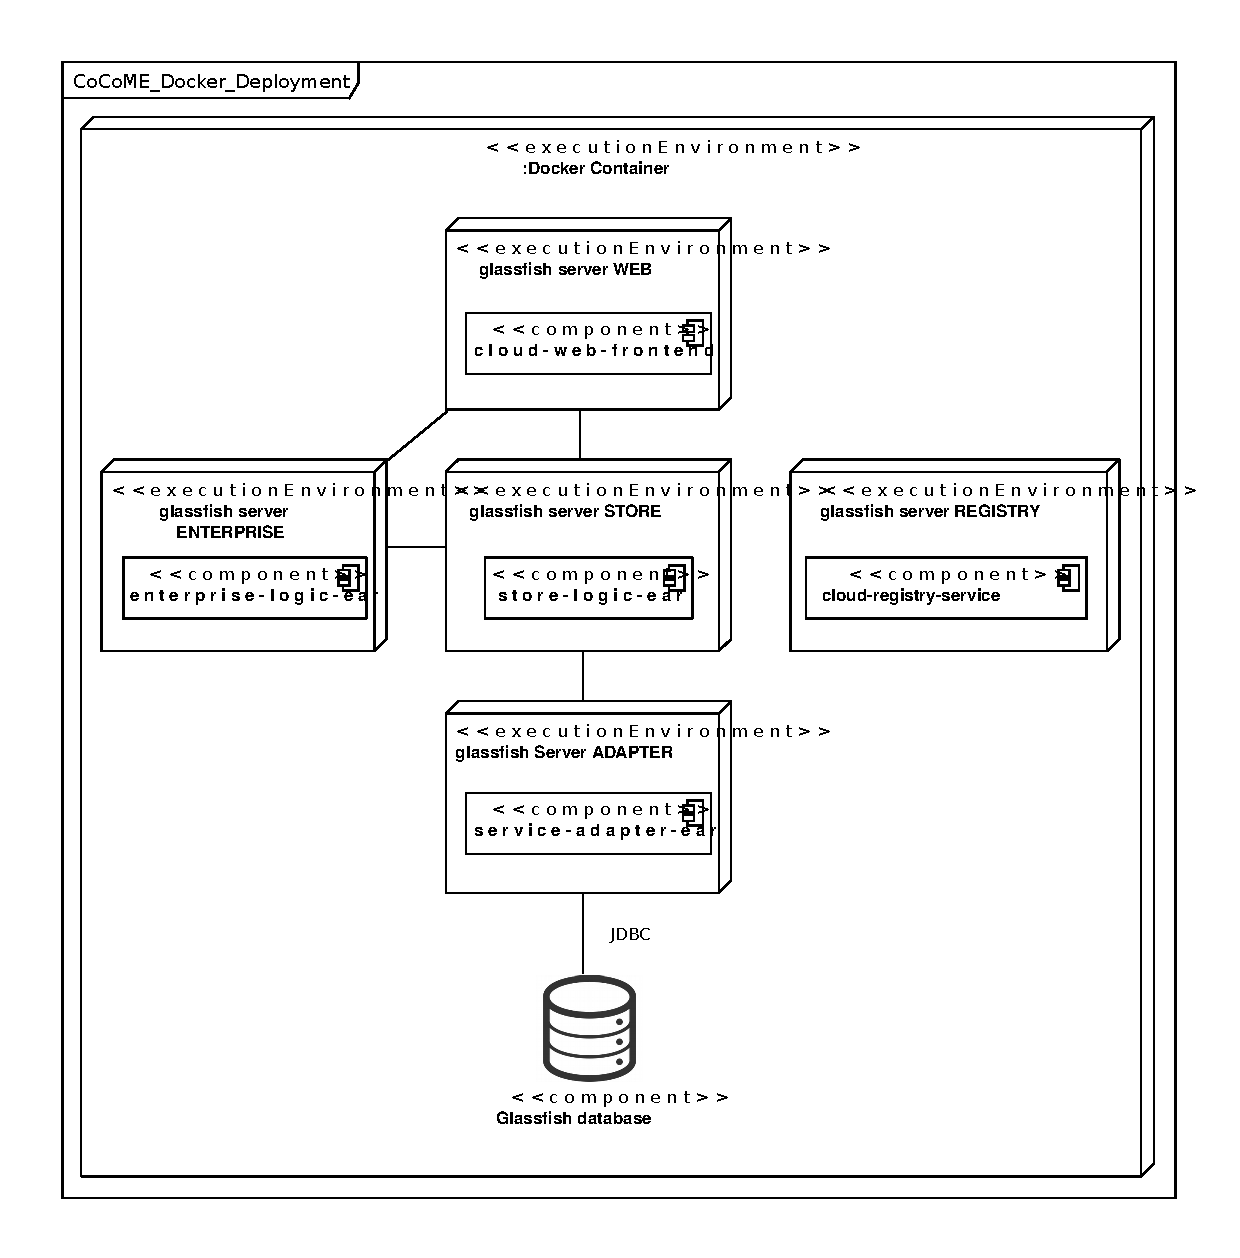
\includegraphics[width = 0.8\textwidth]{img/docker_Container_Deployment.pdf}
 		\caption{Deployment diagram CoCoME}
 		\label{Deploym_CoCoME}
 	\end{figure}
 	\noindent
 	The deployment assignment within the Docker environment is identical to the one specified in CoCoME deployment guide.
 	This means the maven generated archive files \textit{cloud-web-frontend}, \textit{enterprise-logic-ear}, \textit{store-logic-ear}, \textit{cloud-registry-sevice}, and \textit{service-adapter-ear} are deployed on the servers by using the following assignment:
 	\begin{figure}[H]
 		\centering
 		\begin{tabular}{l| l l}%'{p{0.25\textwidth}|p{0.01\textwidth}p{0.25\textwidth}}
 			Server && Deployment file \\
 			\hline
 			WEB && cloud-web-frontend  \\
 			ENTERPRISE && enterprise-logic-ear  \\
 			STORE && store-logic-ear  \\
 			REGISTRY && cloud-registry-service  \\
 			ADAPTER && service-adapter-ear \\	
 		\end{tabular}
 		\caption{Assignment of archive files to \added{the Glassfish }Servers}
 		\label{table_assignment}
 	\end{figure}
 \noindent
    As mentioned earlier, there are two versions of this Docker project.
 	 The fast version can be extended by the Pick-Up shop\footnote{\url{https://github.com/cocome-community-case-study/cocome-cloud-jee-web-shop}}. This Pick-Up shop runs inside a separate Docker container which is shown in Fig.~\ref{Deploym_Pickup}.  
 	\begin{figure}[h]
 		\centering
 		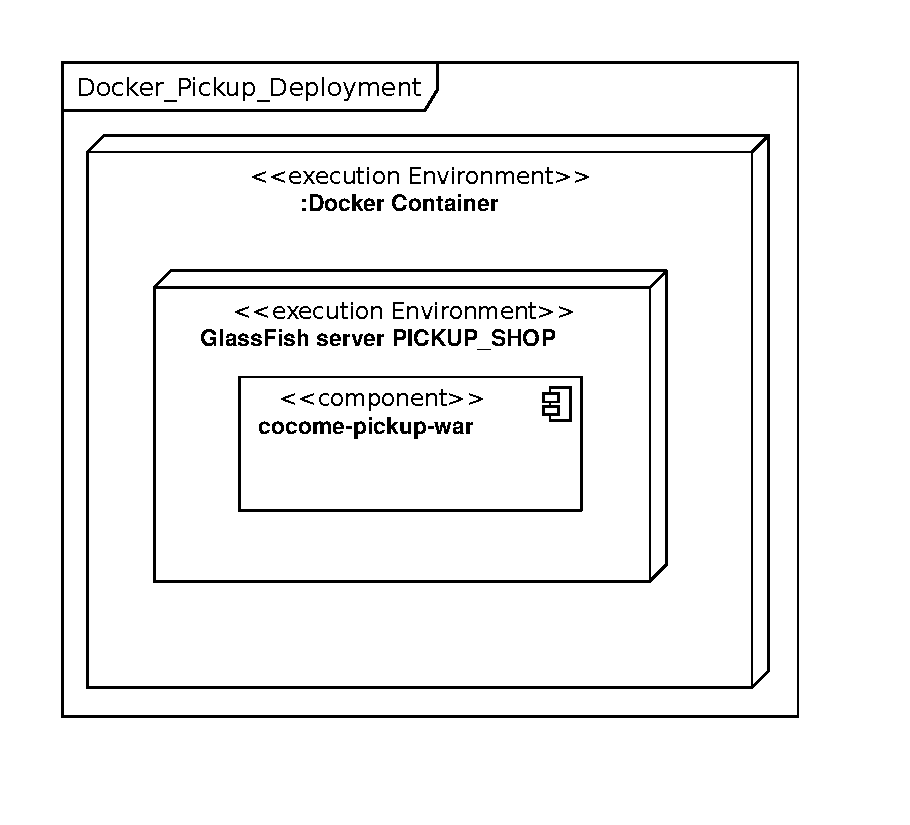
\includegraphics[width = 0.4\textwidth]{img/docker_Container_PickUP.pdf}
 		\caption{Deployment diagram CoCoME Pickup Shop}
 		\label{Deploym_Pickup}
 	\end{figure}
 	As shown in Fig.~\ref{Deploym_Pickup}, this container provides \deleted{only }one Glassfish server.
 	\begin{figure}[H]
 		\centering
 		\begin{tabular}{l|l l}%{p{0.25\textwidth}|p{0.01\textwidth}p{0.25\textwidth}}
 			Server && Deployment file \\
 			\hline
 			PICKUP\_SHOP && cocome-pickup-war \\	
 		\end{tabular}
 		\caption{Assignment \added{of }archive files to \added{the Glassfish }Server\deleted{s}}
 		\label{table_assignment_pickup}
 	\end{figure}
 \noindent
To control the start of both containers, precisely the CoCoME and the Pick-Up Shop, another \deleted{specific} file is needed: the Docker Compose file. 
It ensures that the CoCoME Container is active, before the Pick-Up Shop container starts. 
This is necessary as the Pickup Shop requires a running instance of CoCoME to register itself.\\
Whereas \CoCoME does not require the Pick-Up Shop, the \deleted{inversion}\added{Pick-Up Shop requires \CoCoME.}\deleted{ is not correct.}
Both containers need to communicate with each other. 
By default, \deleted{d}\added{D}ocker prohibits any outgoing and ingoing communication from and in a container. 
This is solved by opening specific ports through which the communication is possible. 
Which ports the containers can use is specified in the Docker Compose file as well.
 	
 	
\section{Adding a Mobile App Client}\label{AppImplementation}
Adding a Mobile App Client \deleted{did}added{does} not require a modification within the hybrid cloud-based variant of CoCoME. 
The implementation was done using the Cordova framework and OnsenUI to provide a multi OS compatible Backend and UI \cite{schnabel}. 
The App itself is written in Typescript/Javascript. 
Fig.\added{~}\ref{App_ClassDiagram} shows the \deleted{principal}\added{primary} classes and their relationships.

The \textit{Navigator} is the primary class that manages the pages. 
The pages consist of two components: The \textit{Page} itself and its \textit{PageState}. 
The \textit{PageState} is used to store and transfer the current status of a page. 
There are currently six different pages available: \textit{IndexPage}, \textit{SearchPage}, \textit{ItemPage}, \textit{CheckoutPage}, \textit{CartPage} and \textit{LoginPage}. 
For the sake of clarity, they are subsumed under the generic terms \textit{ConcretePage} and \textit{ConcretePageState}. 

Pages use components. 
Such components are \deleted{i.e.}\added{for instance} the \textit{Navbar} or the \textit{Searchbar}. 
These components are abstract descriptions of UI elements that are connected to the actual \textit{HTML-elements} via Knockout.js. 
By using Knockout.js, changing values of a component results in an immediate change of the UI. 
Besides, the App Client retrieves information of the CoCoME system.  
As mentioned in \ref{DesignMobileApp}, the Client is not able to access the CoCoME system directly. 
Therefore, the pages use \textit{Services} provided by a \textit{ServiceHolder} to call the \textit{AppController's} \deleted{Rest}\added{REST}-API. 
The \textit{AppController} is written in Java using the SpringBoot framework and converts the \deleted{Rest}\added{REST}-requests of the App Client to SOAP-Requests in order to match the CoCoME-API. 
  
  
   \begin{sidewaysfigure}[ht]
  	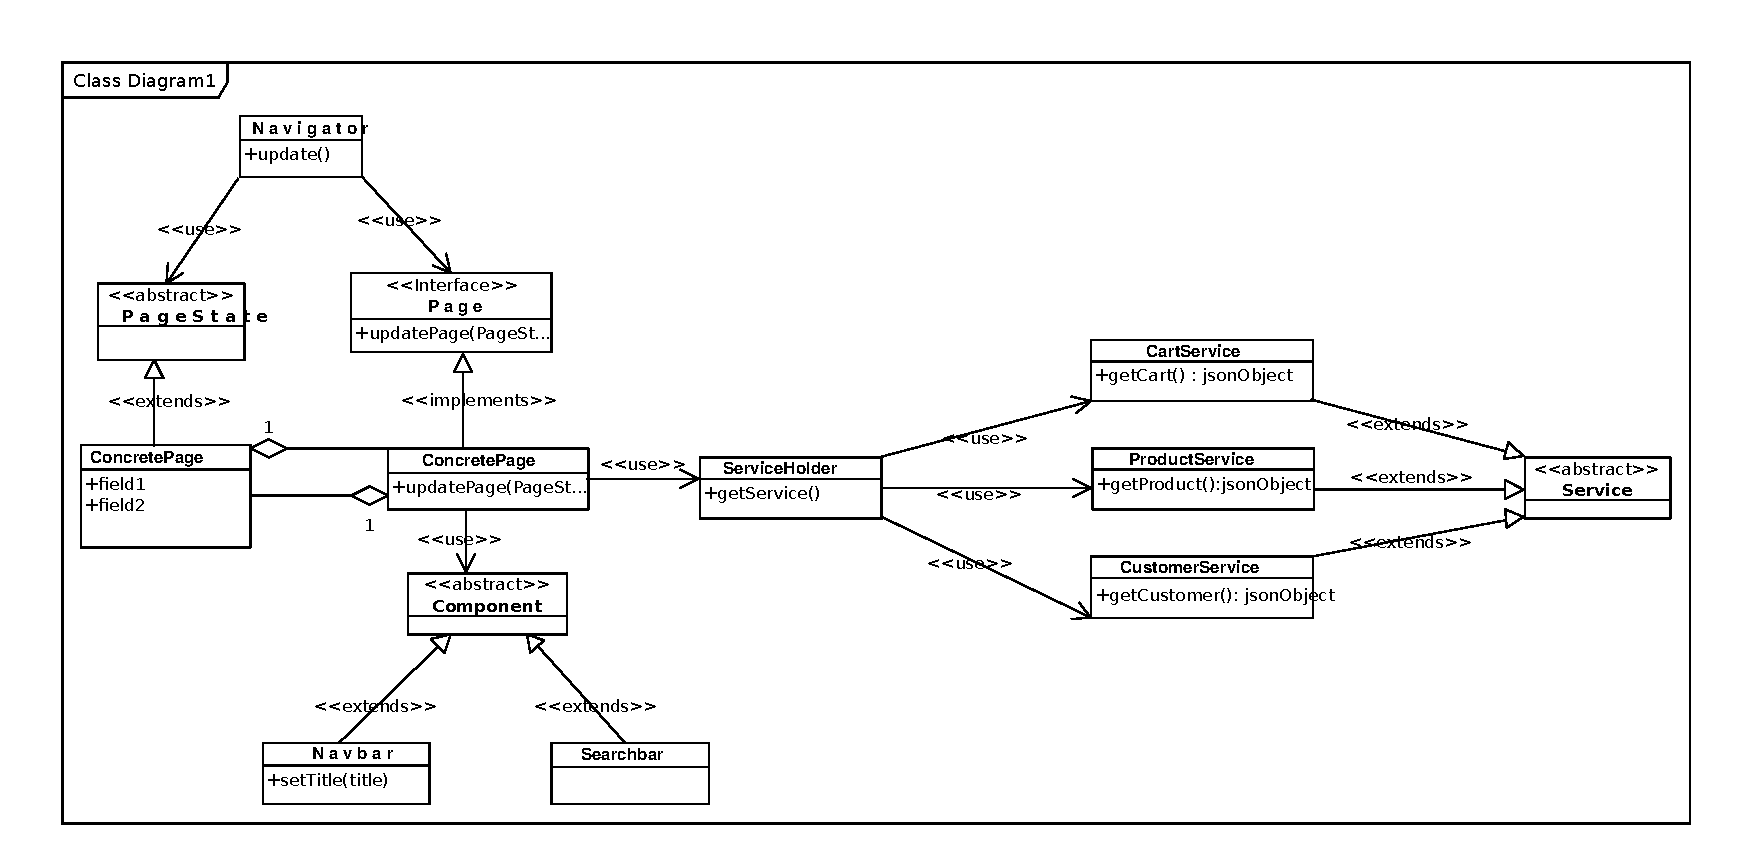
\includegraphics[width=\textwidth]{img/appBasicClass.pdf}
  	\caption{Primary Classes of the App}
  	\label{App_ClassDiagram}
  \end{sidewaysfigure}

\FloatBarrier
 
 
 \section{Using Microservice Technology} \label{MicroserviceImplementation}
 The Microservice evolution scenario of CoCoME transfers the functionality of the hybrid cloud-based variant of CoCoME into a Microservice architecture.
 \added{The service}\deleted{that} is using REST communication between the different services. 
 The implementation is done using Java EE as programming language and Glassfish as deployment server. 
 The Java Persistence API is used to store elements in a relational DB. 
 The Java API for RESTful Web Services (JAX-RS) is used to standardize the REST-communication between the different \deleted{M}\added{m}icroservices. 
 To serialize and deserialize Java-classes to XML- or JSON-files, the Java Architecture for XML Binding (JAXB) is used. 

 Fig.\added{~}\ref{projectStructure} demonstrates the project structure of the \textit{Store} \deleted{M}\added{m}icroservice. 
 The other services have the same structure. 
 Therefore, they are not shown explicitly.  
 Each service project contains three sub-projects, namely \textit{name}-service-ejb, \textit{name}-service-rest and \textit{name}-service-ear. 
 The first sub-project contains the core logic as well as the persistence functionality. 
 The second one provides the RESTful webservice. 
 The last one is used for packaging the projects to ear files. 
 
 
 

 
	\begin{figure}[h]
		\centering
		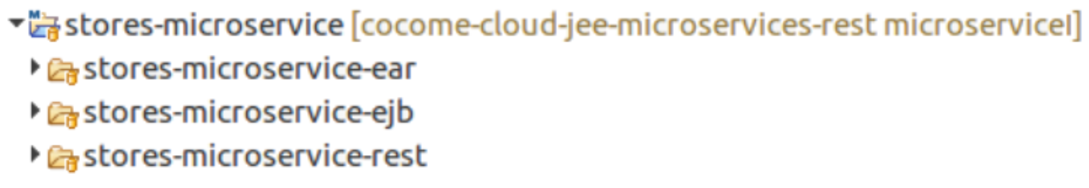
\includegraphics[width = 0.8\textwidth] {img/projectStructure_Micro.pdf}
	 	\caption{Project structure Microservices}
	 	\label{projectStructure}
	 	
 	\end{figure}
 	
